%%%%%%%%%%%%
%
% $Autor: Wings $
% $Datum: 2019-03-05 08:03:15Z $
% $Pfad: TemplateSensor $
% $Version: 4250 $
% !TeX spellcheck = en_GB/de_DE
% !TeX encoding = utf8
% !TeX root = filename 
% !TeX TXS-program:bibliography = txs:///biber
%
%%%%%%%%%%%%

% Structure
\chapter{SG90 Servomotor}

\section*{Einleitung}
Dieses Kapitel beschreibt den mechanischen Aktor des Systems, den Micro-Servomotor TowerPro SG90. Es werden die technischen Spezifikationen, die hardwareseitige Einbindung sowie die softwareseitige Ansteuerung über die Standard-Bibliotheken detailliert erläutert.


\section{Allgemeines}
Ein Servomotor ist ein geschlossenes mechatronisches System (Closed-Loop), das für präzise Winkelpositionierungen eingesetzt wird. Im Gegensatz zu kontinuierlich drehenden Gleichstrommotoren besteht ein Standard-Servo aus einem DC-Motor, einem Untersetzungsgetriebe, einem Potentiometer zur Positionserfassung und einer Steuerelektronik. Der Mikrocontroller sendet ein Pulsweitenmodulations-Signal (\textit{PWM}), welches die Steuerelektronik auswertet und den Motor exakt auf den gewünschten Winkel dreht und dort aktiv hält. Servomotoren findet man vor allem im RC-Modellbau (z.B. Lenkung, Ruder, Klappen), in Robotergelenken sowie in Schwenkmechanismen für Kameras oder Sensoren, bei denen wiederholgenaue und stabile Positionen erforderlich sind.\cite{SparkFun:2026}

\section{Servomotor TowerPro SG90}
Der TowerPro SG90 ist einer der weltweit am häufigsten verwendeten Micro-Servomotoren für kleine Projekte. Er zeichnet sich durch sein extrem geringes Gewicht, seine kompakte Bauform und sein Nylon-Zahnradgetriebe aus. Der Aktor verfügt über ein dreipoliges Anschlusskabel: Braun für die Masse (\textit{GND}), Rot für die Versorgungsspannung (\textit{VCC}) und Orange für das PWM-Steuersignal (\python{Signal}). Der TowerPro SG90 hat einen mechanischen Rotationsspielraum von 180 Grad ($0^\circ$ bis $180^\circ$). Gesteuert wird er über ein 50-Hz-PWM-Signal (20 ms Periodendauer). Eine Pulsweite von 1 ms entspricht theoretisch $0^\circ$, 1,5 ms entsprechen $90^\circ$ (Mittelstellung) und 2 ms entsprechen $180^\circ$.\cite{Elektronik:2026,Components101:2026}  

\section{Spezifikation}
\begin{itemize}
	\item \textbf{Quellen referenzieren:} Die physikalischen und elektrischen Kennwerte beziehen sich auf technische Angaben zum SG90 von Elektronik-Kompendium und Components101.\cite{Elektronik:2026,Components101:2026}
	\item \textbf{Extrahierte Informationen:}
	\begin{itemize}
		\item Betriebsspannung: 4,8 V (ca. 5 V)
		\item Stellmoment (Stall Torque): 1,8 kg/cm (bei 4,8 V)
		\item Stellgeschwindigkeit (ohne Last): 0,1 Sekunden / 60 Grad (bei 4,8 V)
		\item Gewicht: 9 Gramm
		\item Getriebetyp: Kunststoff (Nylon)
		\item Steuersignal: PWM (50 Hz / 20 ms Periode)
		\item Dimensionen: ca. 22,2 x 11,8 x 31 mm 
	\end{itemize}
	
	\begin{figure}[htbp]
		\centering
		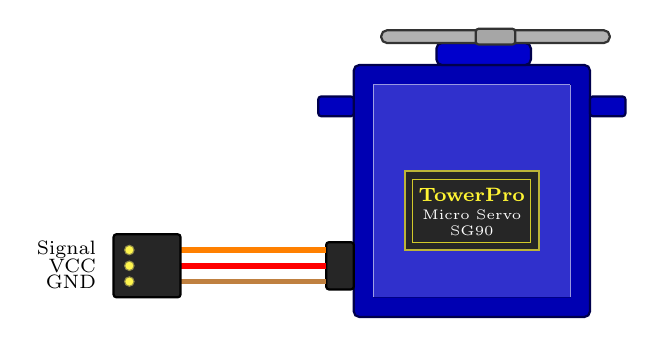
\begin{tikzpicture}[scale=1]
	
	% Hauptgehäuse
	\draw[fill=blue!70!black, draw=blue!30!black, thick, rounded corners=2pt]
	(0,0) rectangle (3.0,3.2);
	
	% Leichte transparente Innenfläche
	\draw[fill=blue!45, draw=blue!20!black, opacity=0.35]
	(0.25,0.25) rectangle (2.75,2.95);
	
	% Schmale Befestigungslaschen oben seitlich
	\draw[fill=blue!75!black, draw=blue!30!black, thick, rounded corners=1pt]
	(-0.45,2.55) rectangle (0,2.80);
	
	\draw[fill=blue!75!black, draw=blue!30!black, thick, rounded corners=1pt]
	(3.0,2.55) rectangle (3.45,2.80);
	
	% Oberes Getriebegehäuse, kleiner
	\draw[fill=blue!80!black, draw=blue!30!black, thick, rounded corners=2pt]
	(1.05,3.2) rectangle (2.25,3.48);
	
	% Servoarm als seitlich betrachteter Rotorarm, länger und ohne Löcher
	\draw[fill=gray!60, draw=gray!40!black, thick, rounded corners=2pt]
	(0.35,3.48) rectangle (3.25,3.64);
	
	% Kleine zentrale Verdickung des Arms
	\draw[fill=gray!70, draw=gray!40!black, thick, rounded corners=1pt]
	(1.55,3.46) rectangle (2.05,3.66);
	
	% Frontlabel
	\draw[fill=black!85, draw=yellow!70!black, line width=0.7pt]
	(0.65,0.85) rectangle (2.35,1.85);
	
	\draw[draw=yellow!80!black, line width=0.4pt]
	(0.75,0.95) rectangle (2.25,1.75);
	
	\node[text=yellow!80!white, font=\scriptsize\bfseries] at (1.5,1.55) {TowerPro};
	\node[text=white, font=\tiny] at (1.5,1.30) {Micro Servo};
	\node[text=white, font=\tiny] at (1.5,1.10) {SG90};
	
	% Gehäusekanten / transparente Details
	\draw[blue!20!white, line width=0.5pt, opacity=0.75]
	(0.25,0.25) -- (0.25,2.95);
	
	\draw[blue!20!white, line width=0.5pt, opacity=0.75]
	(2.75,0.25) -- (2.75,2.95);
	
	\draw[blue!20!white, line width=0.5pt, opacity=0.75]
	(0.25,2.95) -- (2.75,2.95);
	
	% Kabelausgang links unten
	\draw[fill=black!85, draw=black, thick, rounded corners=1pt]
	(0,0.35) rectangle (-0.35,0.95);
	
	% Kabel nach links
	\draw[brown, line width=2pt]
	(-0.35,0.45) -- (-2.2,0.45);
	
	\draw[red, line width=2pt]
	(-0.35,0.65) -- (-2.2,0.65);
	
	\draw[orange, line width=2pt]
	(-0.35,0.85) -- (-2.2,0.85);
	
	% Stecker links
	\draw[fill=black!85, draw=black, thick, rounded corners=1pt]
	(-3.05,0.25) rectangle (-2.2,1.05);
	
	% Kontakte am Stecker
	\draw[fill=yellow!70!white, draw=yellow!50!black]
	(-2.85,0.45) circle (0.06);
	
	\draw[fill=yellow!70!white, draw=yellow!50!black]
	(-2.85,0.65) circle (0.06);
	
	\draw[fill=yellow!70!white, draw=yellow!50!black]
	(-2.85,0.85) circle (0.06);
	
	% Kabelbeschriftung links neben dem Stecker
	\node[font=\scriptsize, anchor=east] at (-3.15,0.45) {GND};
	\node[font=\scriptsize, anchor=east] at (-3.15,0.65) {VCC};
	\node[font=\scriptsize, anchor=east] at (-3.15,0.85) {Signal};
	
\end{tikzpicture}
		\caption{Schematische Darstellung des Servomotors TowerPro SG90}
		\label{fig:sg90_tikz}
	\end{figure}
	
	\item \textbf{Schaltplan:} Das rote Kabel (\textit{VCC}) des SG90 wird mit dem 5V-Ausgang (\textit{VUSB}) des Systems verbunden, um ausreichend Leistung für den Motor bereitzustellen. Das braune Kabel (\textit{GND}) wird mit der gemeinsamen Masse verbunden. Das orange Kabel (\textit{Signal}) wird an einen digitalen PWM-fähigen Pin (z.B. Pin 9) des Mikrocontrollers angeschlossen.\cite{Elektronik:2026} 
	
	\textit{Hinweis:} Der Arduino Nano 33 BLE Sense arbeitet mit 3,3V-I/O-Pegeln und ist nicht 5V-tolerant.\cite{ArduinoNano:2026} 
	Viele Servomotoren können jedoch ein 3,3V-PWM-Steuersignal verarbeiten, sofern der Servo selbst mit einer geeigneten Versorgungsspannung betrieben wird und eine gemeinsame Masse vorhanden ist.\cite{DroneBot:2026}
\end{itemize}

\section{Bibliothek}

\subsection{Beschreibung}
Für die Ansteuerung des SG90 wird in der Arduino-Umgebung die integrierte
\textit{Servo}-Bibliothek genutzt\cite{ArduinoServo:2025}. Dadurch entfällt für den Programmierer die aufwändige Erzeugung des exakten 50-Hz-PWM-Signals, und der Motor kann bequem über die direkte Vorgabe eines Winkelwertes von 0 bis 180 Grad angesteuert werden.\cite{ArduinoServo:2025}

\subsection{Installation}
\begin{itemize}
	\item \textbf{Installation:} Die Bibliothek kann in der Arduino IDE über den Bibliotheksverwalter eingebunden werden. Im Programm wird sie anschließend mit \PYTHON{\#include <Servo.h>} importiert.\cite{SparkFun:2026}

	\item \textbf{Data types:} Die Zielwinkel werden als \python{int} (Integer/Ganzzahlen) übergeben. Für präzisere Steuerungen können Pulsweiten in Mikrosekunden ebenfalls als \python{int} übergeben werden (vgl. \cite{ArduinoServo.h:2025}).
	\item \textbf{Data structure:} Jeder Servomotor wird im Code als Objekt der Klasse \textit{Servo} deklariert (z.B. \PYTHON{meinServo;}).
	\item \textbf{Data quantity:} Auf Standard Arduino-Boards unterstützt die Bibliothek bis zu 12 Servos gleichzeitig; auf speziellen Architekturen (wie der Mbed-OS Architektur des Nano 33 BLE) kann dies variieren, reicht jedoch für mehrere Aktoren vollkommen aus.\cite{ArduinoServoRef}
	\item \textbf{Data quality:} Die Bibliothek arbeitet timer- und interruptbasiert. Die Servosignale werden im Hintergrund mit dem zuletzt über \PYTHON{write()} gesetzten Wert erzeugt, wodurch keine manuelle PWM-Erzeugung mit blockierenden Delay-Schleifen notwendig ist.\cite{ArduinoServo.h:2025}
\end{itemize}

\subsection{Funktionen}
Die wichtigsten Methoden der Bibliothek sind:
\begin{itemize}
	\item \PYTHON{attach(pin)}: Verbindet das Servo-Objekt mit einem bestimmten digitalen Pin.\cite{ArduinoAttach}
	\item \PYTHON{write(angle)}: Dreht den Servo auf den entsprechenden Winkel ($0^\circ$ bis $180^\circ$).
	\item \PYTHON{writeMicroseconds(uS)}: Ermöglicht die Ansteuerung über Pulsweiten in Mikrosekunden.\cite{ArduinoWr}
	\item \PYTHON{read()}: Gibt den zuletzt gesetzten Servo-Winkel zurück.\cite{Arduino}
\end{itemize}

\section{Beispiel}
Dieser Abschnitt zeigt ein elementares Beispiel "`Sweep"', bei dem der Servo kontinuierlich von 0 auf 180 Grad und wieder zurück schwenkt.

\subsection{Handbuch}
Schlie\ss en Sie das rote Kabel an 5V, das braune an GND und das orange Signalkabel an Pin 9 des Arduinos an. Kompilieren Sie das Programm und laden Sie es auf das Board. Der Arm des Servomotors sollte nun anfangen, langsam und gleichmäßig hin und her zu wischen.\cite{ArduinoServoGitHub}

\subsection{An einem Beispiel}
Das Skript in \ref{BeispielCode} bindet zunächst die Bibliothek \PYTHON{Servo.h} ein und erstellt mit \PYTHON{radarServo} ein Servo-Objekt. Zusätzlich wird die Variable \PYTHON{pos} zur Speicherung der aktuellen Winkelposition verwendet. In der \textit{setup()}-Routine wird der Motor über \PYTHON{radarServo.attach(9)} an den digitalen Pin 9 gebunden.

In der \textit{loop()}-Schleife sorgen zwei \PYTHON{for}-Schleifen für die kontinuierliche Schwenkbewegung des Servomotors. Die erste Schleife erhöht den Winkel schrittweise von 0° auf 180°. Dabei wird mit \PYTHON{radarServo.write(pos)} jeweils eine absolute Zielposition angefahren. Nach jeder Winkeländerung folgt mit \PYTHON{delay(15)} eine kurze Pause von 15 ms, damit der Motor die physikalische Position erreichen kann. Die zweite Schleife führt anschließend die Rückwärtsbewegung von 180° zurück auf 0° aus. Dadurch entsteht eine fortlaufende Hin- und Herbewegung des Servomotors.

\subsection{Code}
\begin{center}
	\captionof{code}{Beispiel Code für den TowerPro SG90} \label{BeispielCode} \ArduinoExternal{}{../../Code/Servomotor/Servomotor.ino} 
\end{center}

\subsection{Dateien}
Für das Ausführen des Codes wird ausschlie\ss lich die Standard-Headerdatei \python{Servo.h} benötigt, welche in der Arduino IDE vorinstalliert ist.

\section{Kalibrierung}
Oftmals weichen günstige SG90-Motoren mechanisch von den theoretischen PWM-Werten ab (1000 \textmu s bis 2000 \textmu s). Wird der Motor mit \PYTHON{write(0)} oder \PYTHON{write(180)} an seine physischen Grenzen gezwungen, kann er brummen, vibrieren und überhitzen (Stalling). Zur Kalibrierung bietet die \python{attach()}-Funktion optionale Parameter für die minimalen und maximalen Mikrosekunden: \PYTHON{radarServo.attach(9, 500, 2400);}. Diese Werte müssen durch iteratives Ausprobieren (mit \PYTHON{writeMicroseconds()}) an den individuellen Motor angepasst werden, bis der volle $180^\circ$-Winkel ohne mechanisches Blockieren erreicht ist.\cite{ArduinoAttach,ArduinoWriteMicroseconds}

\section{Einfacher Code (ohne Bibliothek)}
Der Code in \ref{CodeohneBib} erzeugt das PWM-Signal für den Servo manuell ohne die Verwendung der Servo-Bibliothek. In der \textit{setup()}-Routine wird Pin 9 mit \PYTHON{pinMode(9, OUTPUT)} als Ausgang konfiguriert. Die \textit{loop()}-Funktion generiert anschlie\ss end ein 50-Hz-Signal. Dazu wird der Pin mit \PYTHON{digitalWrite(9, HIGH)} für 1500~\textmu s auf HIGH gesetzt, was ungefähr einer Servo-Position von $90^\circ$ entspricht. Danach wird der Pin mit \PYTHON{digitalWrite(9, LOW)} für 18500~\textmu s auf LOW gesetzt, sodass eine vollständige Periodendauer von 20~ms entsteht.

Diese Methode zeigt vereinfacht, wie die Ansteuerung eines Servomotors über ein PWM-Signal funktioniert. Da der Ablauf jedoch durch die verwendeten Verzögerungen blockierend ist, eignet sich diese Variante nur eingeschränkt für komplexere Anwendungen. In solchen Fällen sollte die Servo-Bibliothek verwendet werden, da diese mit Timern arbeitet und die Ansteuerung komfortabler übernimmt.

\begin{center}
	\captionof{code}{Code ohne Bibilothek für den TowerPro SG90} \label{CodeohneBib} 
	\ArduinoExternal{}{../../Code/Servomotor/ServomotorohneBib.ino} 
\end{center}

\section{Einfache Anwendung}
Eine klassische Anwendung für den SG90 ist die Basis eines \textbf{Ultraschall-Radarsystems} (wie im vorliegenden Projekt). Der Ultraschallsensor HC-SR04 wird auf der Achse des Servos montiert. Der Servo tastet systematisch in 1-Grad-Schritten die Umgebung vor sich ab ($0^\circ$ bis $180^\circ$). Bei jedem Schritt wird eine Entfernungsmessung durchgeführt. Diese Kombination aus Aktor-Winkel und Sensor-Distanz ermöglicht es der Software (z. B. in Processing), eine zweidimensionale "`Radarkante"' der Umgebung auf dem Bildschirm zu zeichnen.\cite{ArduinoProjectHubRadar}

\section{Tests}

\subsection{Einfacher Funktionstest}
Mit dem "`Sweep"'-Code aus Abschnitt \ref{CodeohneBib} lässt sich leicht prüfen, ob der Motor korrekt verkabelt ist. Der Motor muss ruckelfrei und flüssig schwenken. Ein stotternder Motor oder ein Neustart des Arduinos während der Bewegung deutet auf eine unzureichende Stromversorgung (VCC-Abfall) hin.

\subsection{Alle Funktionen testen}
Ein vollständiger Systemtest umfasst:


1. \textbf{Grenztest:} Anfahren von $0^\circ$ und $180^\circ$. Der Motor darf in diesen Endlagen nicht surren oder ungewöhnlich warm werden.

2. \textbf{Geschwindigkeitstest:} Befehle \PYTHON{write(0)} und sofort danach \PYTHON{write(180)} ohne Delay. Messung, ob der Motor die physikalische Herstellerangabe von 0,3 Sekunden für diesen $180^\circ$-Weg einhalten kann.

3. \textbf{Präzisionstest:} Verwendung von \PYTHON{writeMicroseconds(1500)} zur exakten Zentrierung, gefolgt von der Überprüfung der Winkelgenauigkeit mittels eines Geodreiecks auf dem Rotorkopf.

\section{Weiterführende Literatur}

\begin{thebibliography}{9}
	
	\bibitem{ArduinoAttach}
	ArduinoGetStarted: \textit{Servo.attach() | Arduino Reference}. Verfügbar unter:
	\url{https://arduinogetstarted.com/reference/library/servo-attach}
	[abgerufen am 10.05.2026]
	
	\bibitem{ArduinoWriteMicroseconds}
	ArduinoGetStarted: \textit{Servo.writeMicroseconds() | Arduino Reference}. Verfügbar unter:
	\url{https://arduinogetstarted.com/reference/library/servo-writemicroseconds}
	[abgerufen am 10.05.2026]
	
	\bibitem{ArduinoProjectHubRadar}
	Arduino Project Hub: \textit{Building an Ultrasonic Radar using Arduino and Processing}. Verfügbar unter:
	\url{https://projecthub.arduino.cc/diegogalvan_1294/building-an-ultrasonic-radar-using-arduino-and-processing-59053e}
	[abgerufen am 10.05.2026]
\end{thebibliography}
